
\chapter{Signal Processing}
After code generation the binary data needs to be transormed into a transmittable signed signal


\section{Pulse shaping}

The raw code which was previously generated is first put through an sign function, which sets its mean to zero. The discontinuous signal holds an infinite bandwidth because it consists of rectangular pulses. These pulse spans have infinity frequency, which are impossible to implement for acoustic transmission. Therefore a restriction to a certain bandwidth must be introduced. Such a reduction is possible by applying an low-pass filter.\\
Because limiting the signals bandwidth introduces a damped oscillation, which leads to incorrect decoding of received data \cite{bibid}, a appropriate choice of filter would be a the raised cosine \ref{eq:cosfir}. Such a pulse filter is defined by a squared cosine, which decreases its amplitude in frequency. In our case the roll off factor $\alpha$ is set to $0.125$ and symbol length $T_{sym}$ to the inverse of our target bandwidth $20\,kHz$.\\
Before applying the filter the generated codes need to be up-scaled for our target sampling rate. The relation between sampling rate $f_s$ and up-sampling factor $Sp_s$ is $Sp_s=fs\cdot T_{sym}$.

\begin{equation}
	H(\omega)=T_{sym}\cdot \cos^2\left(\dfrac{T_{sym}(\omega-\pi(1-\alpha)/T_{sym})}{4\alpha}\right),~~~\omega=2\pi f
	\label{eq:cosfir}
\end{equation}


\begin{figure}[h]
	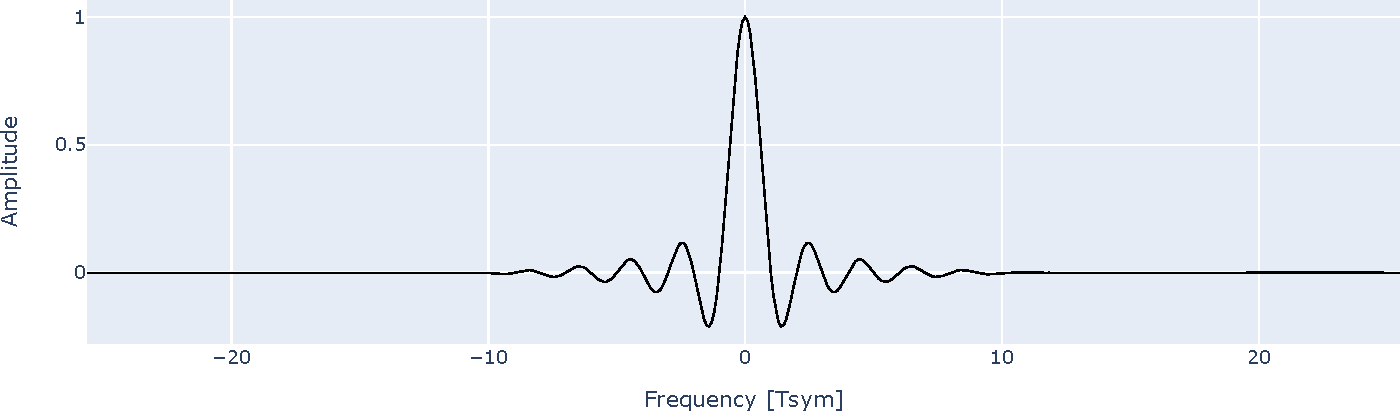
\includegraphics[width=\linewidth]{images/cosfir}
	\caption{Section of Cosine FIR with a resolution of 1024}
	\label{fig:cosfir}
\end{figure}


\section{Shift to Carrier}

Now that our base band signal $tSigBB[k]$ has its target bandwidth and sample rate only the frequency shift to the carrier frequency $f_c$ of $62.5\,kHz$ is necessary. That procedure is accomplished by multiplying our sampled signal by the exponential function, where $f_c$ is passed to its exponent. The resulting signal could hold imaginary parts, hence only the real part is passed through for transmission.\\
The signal is now in a appropriate state for the use inside an localization algorithm, where the delays of the signals can be detected by the help of cross-correlation techniques.
\begin{equation}
	x_{tSigTB}[k]=Re\{x_{tSigBB}[k]\cdot e^{-2\pi j f_c k}\}
	\label{eq:shift}
\end{equation}

%\begin{equation}
%	x_{tSigBB}[k]=x_{tSigTB}[k]\cdot e^{-2\pi j (-f_c) k}
%	\label{eq:rshift}
%\end{equation}

%\section{Simulation}
%The simulation consists of a watermark benchmark \cite{watermark15} and a additive GWN generated by a desired SNR between $-20dB$ and $20dB$ in steps of $5dB$. From the general equation of the Signal to Noise Ratio we derive our noise standard deviation by transforming this ratio. The white noise is added after the simulation and before receiver filtering.
%\begin{equation}
%	SNR=\cfrac{P_{Signal}}{P_{Noise}}=\cfrac{\mathbb{E}({Signal}^2)}{\mathbb{E}({Noise}^2)}=\cfrac{\sum {Signal}^2}{N\cdot\sigma_{Noise}^2}~~\Leftrightarrow~~\sigma_{Noise}=\sqrt{\cfrac{\sum^N {Signal}^2}{N\cdot SNR}}
%\end{equation}
%
%\begin{equation}
%	SNR_{dB}=10\cdot\log_{10}\cfrac{\sum Signal^2}{\sum Noise^2}
%	=10\left(\log_{10}\sum^N_{k=1} x_{TB}^2[k]-\log_{10}\sum^N_{k=1} Noise^2[k]\right)
%\end{equation}
%
%\begin{equation}
%	Noise=\text{\textsc{Normal}}(0,1)\cdot \cfrac{\sigma_{Signal}}{SNR}
%\end{equation}
\begin{figure}[h]
	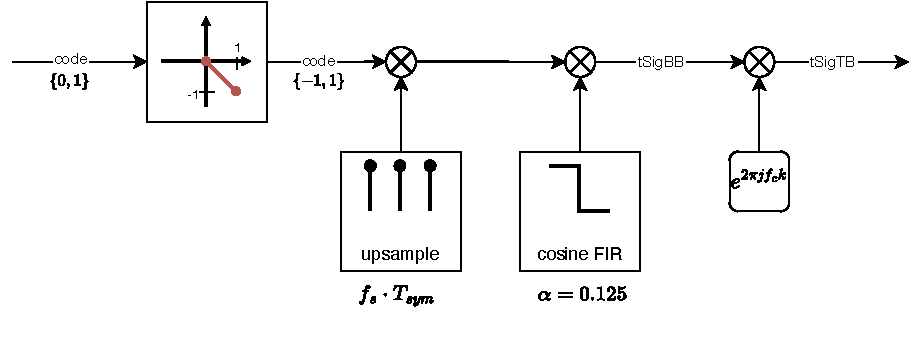
\includegraphics[width=\linewidth]{images/sensig}
	
	\caption{Processing of generated signal}
	\label{fig:sensig}
\end{figure}


\section{Band pass filter}
On the receiver side all signals are received as a sum, which is mixed by artifacts of signal reflections and random noise from the electronics.\\
The received signal may have noise around its bandwidth. Thus, we only pass though frequencies inside our frequency band by applying a butterworth band pass filter.
A flat magnitude is favorable because only frequencies of the base-band should be passed through. 
The filter gets applied after shifting back to the base-band. Such a filter, namely a maximally flat magnitude filter, approximates this goal. The roll-off decreases by increasing the order of the system.\\
The critical frequencies of the applied filter are $f_c\pm\dfrac{bw}{2}$ by an Order of 5. Thus frequencies get removed which are not inside the spectrum of interest. To remove shifts in time the filter is applied forwards and backwards following a doubling of its order.

\section{Shift to base band}

Shifting the transmitted signal back to its original frequency is feasible by just changing its sign. In this case also the imaginary part can be retained.

\begin{equation}
	x_{tSigBB}[k]=x_{tSigTB}[k]\cdot e^{2\pi j f_c k}
	\label{eq:rshift}
\end{equation}

\section{Low-pass Filter}
Because .... The same kind of filter, which was used for pruning the carrier frequencies is used as a low-pass. The same Order and twice filtering principle is used.
\begin{figure}[h]
	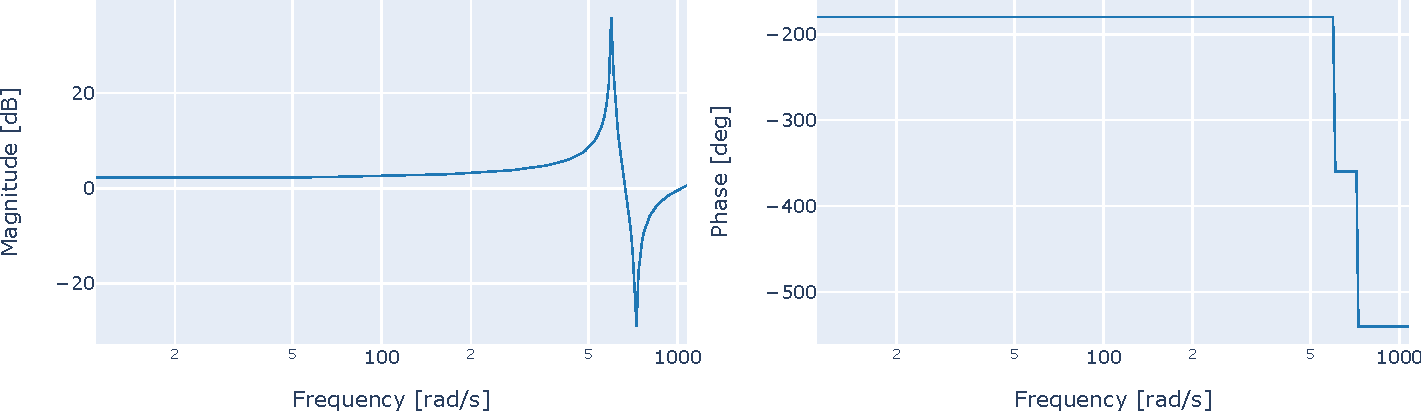
\includegraphics[width=\linewidth]{images/bode}
	
	\caption{Bode plot of 5th order Butterworth low-pass filter}
	\label{fig:bode}
\end{figure}

\begin{figure}[h]
	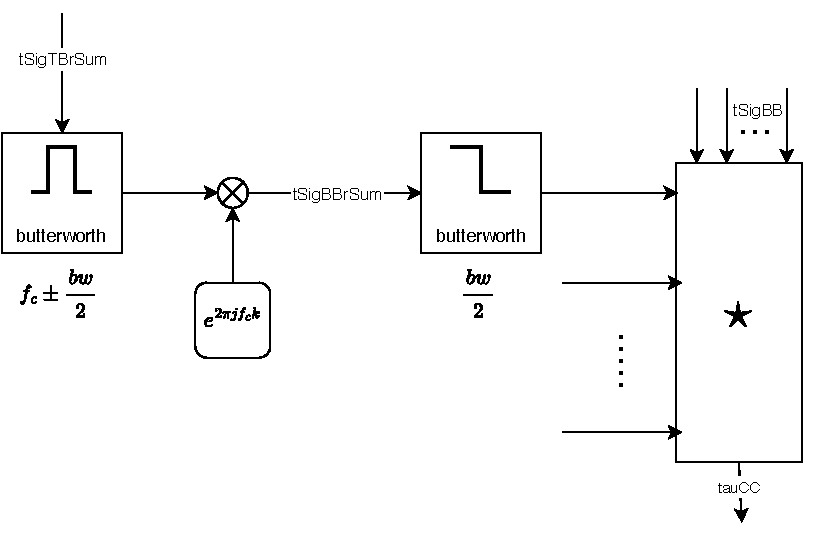
\includegraphics[width=\linewidth]{images/recsig}
	
	\caption{Processing of received signal}
	\label{fig:recsig}
\end{figure}


